\chapter{Introduction to the singlet-doublet fermion DM model}
%
\InitialCharacter{T}he singlet-doublet fermion dark matter model (SDFDM) is introduced in this chapter.  
Its features are described in detail focusing in the contributions to the electroweak precision tests parameters, 
the Higgs and the $Z$ invisible decays, and its prospects for direct and indirect detection of dark matter. Also, it is described the implementation of this model and how the dark matter observables are computed using some high energy tools. At the end, it is shown how to enlarge the model with new reals scalar singlets in order to have radiative massive neutrinos.

\section{The SDFDM model}
\label{sec:model}
%
The SDFDM model has been previously studied in~\cite{D'Eramo:2007ga,Enberg:2007rp,Cohen:2011ec,Calibbi:2015nha,Abdallah:2015ter,Abe:2014gua}.
The particle content of the model consists of two $SU(2)_L$-doublets of
Weyl fermions $\widetilde{R}_u$, $R_d$  with opposite hypercharges and one singlet
Weyl fermion $N$ of zero hypercharge. 
All of them are odd under one imposed $Z_2$ symmetry, under which the SM
particles are even. 
The new particle content is summarized in Table~\ref{tab:partcont}.
%
\begin{table}
  \centering
  \begin{tabular}{|l|l|l|l|}
    \hline  
    Symbol     & $\left( SU(2)_L, U(1)_Y \right)$ & $Z_2$ & \text{Spin}\\ \hline
    $N$  & $(1,0)$ & $-$ & 1/2\\
     $\widetilde{R}_u$, & $(2, +1/2)$ & $-$ & 1/2\\ 
     $R_d$ & $(2, -1/2)$ & $-$ & 1/2\\ \hline
  \end{tabular}
  \caption{New $Z_2$-odd Weyl fermions in the SDFDM model.}
  \label{tab:partcont}
\end{table}
%
The most general $Z_2$-invariant Lagrangian is given by
\begin{align}
\label{eq:lt13A}
 \mathcal{L}= &\mathcal{L}_{\text{SM}}+\left[\mathcal{L}_{\text{Kin}}+ M_D \epsilon_{ab}R^a_d \widetilde{R}^b_u-\tfrac{1}{2}M_N NN-\lambda_d\, \epsilon_{ab}H^a R_d^b N-\lambda_u \epsilon_{ab}\widetilde{H}^a \widetilde{R}_u^b N+\text{h.c} \right]\,,
\end{align}
where
\begin{align}\label{eq:weyl-doublets}
  R_{d}=&
  \begin{pmatrix}
    \psi_{L}^{0}\\
    \psi_{L}^{-}
  \end{pmatrix}
&  
\widetilde{R}_{u}=&
  \begin{pmatrix}
   - \left( \psi_{R}^{-} \right)^{\dagger}\\
     \left(\psi_{R}^{0}\right)^{\dagger}
  \end{pmatrix}\,,
\end{align}
and $H=1/\sqrt{2} \begin{pmatrix}-iG^+ & h+v+iG^0\end{pmatrix}^{\operatorname{T}}$ is the SM Higgs doublet with $\widetilde{H}=i\sigma_2H^*$. 

In general, this model has four complex parameters ($-M_D, M_N, \lambda_u, \lambda_d$) of which
three  can be chosen reals with a redefinition of the fermion fields $N$, $R_d$ and $\widetilde{R}_{u}$. 
Therefore, in this work the three parameters  $-M_D$, $M_N,$ and $\lambda_u$ are chosen to be reals and positives. 
The last parameter $\lambda_d$ can be complex, but it was chosen real in order to avoid CP violation~\cite{Abe:2014gua}. 

Expanding the Lagrangian~\eqref{eq:lt13A} is obtained
\begin{align}
\label{eq:lt13a-expanded}
\mathcal{L}  \supset \, & \mathcal{L}_{\text{Kin}}+M_D(R_d^1\widetilde{R}_u^2-R_d^2\widetilde{R}_u^1)-\tfrac{1}{2}M_N NN
-\lambda_d(H^1R_d^2-H^2R_d^1)N-\lambda_u(\widetilde{H}^1R_u^2-\widetilde{H}^2R_u^1)N+\text{h.c}\nonumber \\
=\,& \mathcal{L}_{\text{Kin}}+M_D(\psi_L^0{\psi_{R}^0 }^{\dagger}+\psi_L^-{\psi_{R}^- }^{\dagger})-\tfrac{1}{2}M_N NN
+\dfrac{\lambda_d (h+v)}{\sqrt{2}}\psi_L^0N - \dfrac{\lambda_u (h+v)}{\sqrt{2}}{\psi_R^0}^{\dagger}N +\text{h.c}\nonumber\\
=\,& \mathcal{L}_{\text{Kin}}+\left[M_D\psi_L^0{\psi_{R}^0 }^{\dagger}-\tfrac{1}{2}M_N NN + \dfrac{\lambda_d v}{\sqrt{2}}\psi_L^0N - \dfrac{\lambda_u v}{\sqrt{2}}{\psi_R^0}^{\dagger}N\right]
+ M_D\psi_L^-{\psi_{R}^- }^{\dagger}
\nonumber\\ & 
+ \dfrac{h}{\sqrt{2}}\left(\lambda_d\psi_L^0N - \lambda_u{\psi_R^0}^{\dagger}N\right)+\text{h.c}.
%
\end{align}
%
Therefore, the $Z_2$-odd fermion spectrum in this model is composed of a
charged Dirac fermion $X^{\pm}=(\psi^{\pm}_L,\, \psi^{\pm}_R)^T$ with a tree
level mass $m_{X^\pm}=-M_D$, and three Majorana fermions $X_i^0$ $(i=1,2,3)$ that arise from
the mixture between the two neutral parts of the $SU(2)_L$ doublets and
the singlet fermion, i.e. between $\psi_L^0, \, {\psi_R^0}^{\dagger}$ and $N$. This spectrum will be discussed in the next section.






%%%%%%%%%%%%%%%%%%%%%%%%%%%%%%%%%%%%%%%%%%%%%%%%%%%%%%%%%%%%%%%%%%%%%%%%%%%%%%%%%%%%%%%%%%%%%%%%%%%%%%
\subsection{Neutral mass spectra}
%
Defining the fermion basis through the vector
\begin{align}
\label{eq:vecgauge}
\boldsymbol{\Xi}^{0}=
\begin{pmatrix}
N & R_d^1 & \widetilde{R}_u^2   
\end{pmatrix}^{\operatorname{T}}=
\begin{pmatrix}
N & \psi_L^0 & \psi_R^{0\dagger}
\end{pmatrix}^{\operatorname{T}},
\end{align} 
the mass terms in the Lagrangian~\eqref{eq:lt13a-expanded} can be written as
\begin{align}
\label{eq:neutral_lagrangian}
\mathcal{L}_{\Xi}
=& \left[ M_D\psi_L^0{\psi_{R}^0 }^{\dagger}-\tfrac{1}{2}M_N NN
+\dfrac{\lambda_d v}{\sqrt{2}}\psi_L^0N 
- \dfrac{\lambda_u v}{\sqrt{2}} {\psi_R^0}^{\dagger}N\right] +\text{h.c}\nonumber\\
=&-\dfrac{1}{2}\bigg[M_N NN - M_D(\psi_L^0{\psi_{R}^0 }^{\dagger}+{\psi_{R}^0 }^{\dagger}\psi_L^0)
-\dfrac{\lambda_d v}{\sqrt{2}}(\psi_L^0N+N\psi_L^0) 
+\dfrac{\lambda_u v}{\sqrt{2}} ({\psi_R^0}^{\dagger}N+N{\psi_R^0}^{\dagger})\bigg] +\text{h.c}
\nonumber\\
  =&-\frac{1}{2}
\boldsymbol{\Xi}^{0\operatorname{T}}
\mathbf{M}^{\chi}\boldsymbol{\Xi}^0
+\text{h.c}\,,
\end{align}
where
\begin{align}
\label{eq:Mchis}
  \mathbf{M}^{\chi}=\begin{pmatrix}
  M_N                 &-\dfrac{\lambda_d v}{\sqrt{2}}&\dfrac{\lambda_u v}{\sqrt{2}}\\
-\dfrac{\lambda_d v}{\sqrt{2}} &  0                  & -M_D\\
\dfrac{\lambda_u v}{\sqrt{2}}&  -M_D                &  0  \\
\end{pmatrix}\,.
\end{align} 
By defining
%%%%%%%%%%%%%%%%%%%%%%%%%%%%%%%%%%%%%%%%%%%%%%%%%%%%%%%%
\begin{align}
  \label{eq:etabeta}
m_{\lambda}=&  \frac{\lambda v }{\sqrt{2}}\,,&
  \lambda=&\sqrt{\lambda_u^2+\lambda_d^2}\,,&
  \tan\beta=&\frac{\lambda_u}{\lambda_d}\, ,
\end{align}
the neutral fermion mass matrix is given by
\begin{align}
\label{eq:Mchi}
  \mathbf{M}^{\chi}=\begin{pmatrix}
 M_N                 &-m_{\lambda}\cos\beta&m_{\lambda}\sin\beta\\
-m_{\lambda}\cos\beta &  0                  & -M_D\\
m_{\lambda}\sin\beta&  -M_D                &  0  \\
\end{pmatrix}\,,
\end{align}
%
which follow the same
convention of the bino-higgsino sector in the neutralino mass matrix of the
minimal supersymmetric standard model (MSSM)~\cite{Martin:2012us}. 
This convention facilitates the comparison between the present study and previous analysis
regarding the bino-higgsino DM limit of the MSSM. 
Such a limiting scenario occurs in the MSSM when the winos are decoupled from the spectrum and is accommodated within the SDFDM model when
$m_\lambda=m_Z\sin\theta_W$ ($\lambda=g'/\sqrt{2}$).










%%%%%%%%%%%%%%%%%%%%%%%%%%%%%%%%%%%%%%%%%%%%%%%%%%%%%%%%%%%%%%%%%%%%%%%%%%%%%%%%%%%%%%%%%%%%%%%%%
\subsubsection{Neutral mass eigenstates}
In order to get the physics eigenstates, this mass matrix needs to be diagonalized,
in such a way that the fermion mass eigenstates $\mathbf{X}=(\chi_1^0,\chi_2^0,\chi_3^0)^T$ are obtained through the rotation
matrix $\mathbf{N}$\footnote{In~\cite{Horiuchi:2016tqw} was used $\mathbf{U}$ instead $\mathbf{N}$. The equivalence is $\mathbf{N}=\mathbf{U}^T$.} as 

\begin{align}
\label{eq:rotation}
\boldsymbol{\Xi}^0 = \begin{pmatrix}N\\ \psi_L^0 \\ (\psi_R^0)^\dagger\end{pmatrix}= 
\mathbf{N}\begin{pmatrix}\chi_1^0\\ \chi_2^0 \\ \chi_3^0\end{pmatrix}= \mathbf{N}\mathbf{X} \,,
\end{align}
such that

\begin{align}
\label{eq:chidiag}
 \mathbf{N}^{\operatorname{T}}\mathbf{M}^\chi \mathbf{N}=\mathbf{M}^\chi_\text{diag}\,,
\end{align}
%
with $\textbf{M}^\chi_{\text{diag}}=\operatorname{Diag}(m^\chi_1,m^\chi_2,m^\chi_3)$ and $m^\chi_n$ being the corresponding physical masses (not mass ordering is implied). 
Even more, CP invariance is assumed and therefore $\mathbf{N}$ can be chosen real. By using the neutral Lagrangian~\eqref{eq:neutral_lagrangian} and the Eq.~\eqref{eq:rotation} for the rotation, 
it is possible to get the following expressions for the masses
%
\begin{align}
\label{eq:masses_diag}
m^\chi_1=&\tfrac{1}{2}M_NN_{11}^2 - M_D N_{21}N_{31}-\dfrac{\lambda_dv}{\sqrt{2}}N_{11}N_{21}+\dfrac{\lambda_uv}{\sqrt{2}}N_{11}N_{31}\\
m^\chi_2=&\tfrac{1}{2}M_NN_{12}^2 - M_D N_{22}N_{32}-\dfrac{\lambda_dv}{\sqrt{2}}N_{12}N_{22}+\dfrac{\lambda_uv}{\sqrt{2}}N_{12}N_{32}\\
m^\chi_3=&\tfrac{1}{2}M_NN_{13}^2 - M_D N_{23}N_{33}-\dfrac{\lambda_dv}{\sqrt{2}}N_{13}N_{23}+\dfrac{\lambda_uv}{\sqrt{2}}N_{13}N_{33} \,.
\end{align}
%
The analytical diagonalization of the neutral fermion mass matrix is
carried out in Appendix~\ref{sec:analyt-form-mass}. 
It is useful and convenient in some analysis to have approximate expressions in
the limit of small fermion mixing ($m_\lambda\ll M_D,M_N)$. For instance,
expanding the analytical expressions for the eigensystem of
Eq.~\eqref{eq:chidiag} given in Appendix~\ref{sec:analyt-form-mass}
up to order $m_{\lambda}^2$, the fermion masses are given by
%
\begin{align}
\label{eq:ml2}
m^\chi_1=&M_{N} + \frac{M_{D} \sin{\left (2 \beta \right )} + M_{N}}{M_{N}^{2}- M_{D}^{2} }\, m_{\lambda}^{2}+\mathcal{O}\left( m_{\lambda}^4 \right) \nonumber\\
m^\chi_2=&M_{D} + \frac{ \sin(2 \beta ) + 1}{2 \left( M_{D} -  M_{N} \right)}\,m_{\lambda}^{2}+\mathcal{O}\left( m_{\lambda}^4 \right) \nonumber\\
m^\chi_3=&- M_{D} + \frac{ \sin(2 \beta ) - 1}{2 \left( M_{D} + M_{N} \right) }\,m_{\lambda}^{2}+\mathcal{O}\left( m_{\lambda}^4 \right)\,.
\end{align}
Approximate expressions for the mixing matrix are also given in the Appendix~\ref{sec:analyt-form-mass}.











%%%%%%%%%%%%%%%%%%%%%%%%%%%%%%%%%%%%%%%%%%%%%%%%%%%%%%%%%%%%%%%%%%%%%%%%%%%%%%%%%%%%%%%%%%%%%%%%%%%%%%%%%%%
\subsection{The interaction Lagrangian}
%
According to the Lagrangian Eq.~\eqref{eq:lt13a-expanded}, the interaction terms, and the free-fermion Lagrangian  are given by
%
\begin{align}
\label{eq:lint1}
\mathcal{L} \, \supset \, &\mathcal{L}_{\text{Kin}}
- \dfrac{h}{\sqrt{2}}\left(-\lambda_d\psi_L^0N + \lambda_u{\psi_R^0}^{\dagger}N\right)+\text{h.c}\nonumber\\
= \, & \dfrac{i}{2}\left(N^{\dagger}\overline{\sigma}^{\mu}\partial_{\mu}N 
+  R_d^{\dagger}\overline{\sigma}^{\mu}D_{\mu}R_d 
+  \widetilde{R}_u^{\dagger}\overline{\sigma}^{\mu}D_{\mu}\widetilde{R}_u \right)
- \dfrac{h}{\sqrt{2}}\left(-\lambda_d\psi_L^0N + \lambda_u{\psi_R^0}^{\dagger}N+\text{h.c}\right)\,,
\end{align}
%
where $D_{\mu}$ is the SM covariant derivative. 

Although, this Lagrangian is written in terms of Weyl spinors,
in the  Appendix~\ref{sec:lag-interaction}
the Majorana spinors $X_i^0$ and the Dirac spinor $X^{\pm}$  are constructed as
\begin{align}
X_i^0=\begin{pmatrix}
(\chi_{i}^0)_\alpha \\ (\chi_i^{0\dagger})^{\dot{\alpha}}
\end{pmatrix}
=\begin{pmatrix}
N_{ji}\,\boldsymbol{\Xi}^{0}_j \\
N_{ji}^{\dagger}\,\boldsymbol{{\Xi}^{\dagger}}^{0}_j
\end{pmatrix}
\hspace{1.5 cm}
X^{\pm}=\begin{pmatrix}
\chi^{\pm}_{\alpha} \\ {\chi^{\mp}}^{\dagger\dot{\alpha}}
\end{pmatrix}
=\begin{pmatrix}
\psi_L^{\pm} \\
{\psi_R^{\mp}}^{\dagger}
\end{pmatrix}\,,
\end{align}
%
and it is shown that the interaction Lagrangian in terms of four-component spinors is given by
%
\begin{align}
\label{eq:lint4}
\mathcal{L}_{\text{Int}}= & 
-\dfrac{g}{\sqrt{2}}\left(\bar{X}^-\slashed{W}\left(N_{2i}P_L-N_{3i}P_R\right)X_i^0 + \text{h.c}\right)
+ \dfrac{g}{4\cos\theta}\bar{X}_i^0\slashed{Z}\left(N_{2i}N_{2j}-N_{3i}N_{3j}\right)\gamma^5X_j^0 \nonumber\\
+& g\left(\dfrac{2\cos^2\theta_W-1}{2\cos\theta_W}\right)
\bar{X}^-\slashed{Z}X^-
-e\bar{X}^-\slashed{A}X^- 
-\dfrac{1}{\sqrt{2}}h\bar{X}_i^0\left(-\lambda_dN_{2i}N_{1j} + \lambda_uN_{3i}N_{1j}\right)X_j^0\,.
\end{align}
%
In particular, the interaction of the DM particle $X_i^0$ with the $W$, $Z$ and $h$ SM gauge boson is given by 
%
\begin{align}
\mathcal{L^{\chi}}_{\text{Int}}=
-\bar{X}^-\slashed{W}c_{WXX_i}X_i^0
-c_{ZX_iX_j}\bar{X}_i^0\slashed{Z}\gamma^{5}X_j^0
-c_{hX_iX_j}h\bar{X}_i^0X_j^0 \,,
\end{align}
where 
\begin{align}
c_{WXX_i}=& \dfrac{g}{\sqrt{2}}\left(N_{2i}P_L-N_{3i}P_R\right)  \label{eq:cWXXi}\\
c_{ZX_iX_j}=&\frac{g}{4\cos\theta_W}(N_{3i}N_{3j}-N_{2i}N_{2j}) \label{eq:cZXiXj}\\
%problema en el orden
c_{hX_iX_j}=&\frac{1}{\sqrt{2}}(-\lambda_dN_{2i}N_{1j}+\lambda_uN_{3i}N_{1j})\label{eq:cHXiXj}\,,
\end{align}
%
which it is in agreement with the Ref.~\cite{Abdallah:2015ter}.
 
As is usually done, we denote the lightest stable particle in our model by 
$\chi^0\,$~\footnote{Actually, it is the lightest stable Majorana four-component spinor $X_i^0$, which will be denote as $\chi^0$ for simplicity.}, whose couplings with the $Z$ and $h$ gauge bosons can explicitly written as~\cite{Calibbi:2015nha}
\begin{align}
c_{Z\chi^0\chi^0}&=-\frac{m_Z\lambda^2v(m_{\chi^0}^{2}-M_D^2)\cos2\beta}{2(m_{\chi^0}^{2}-M_D^2)^2+\lambda^2v^2\left(2\sin2\beta m_{\chi^0} M_D+m_{\chi^0}^{2}+M_D^2\right)} \,,\label{eq:cZXX}\\
c_{h\chi^0\chi^0}&=-\frac{(M_D\sin 2\beta+m_{\chi^0})\lambda^2v}{M_D^2+\lambda^2v^2/2+2M_N\,m_{\chi^0}-3m_{\chi^0}^{2}}\label{eq:cHXX}\,.
\end{align}










%%%%%%%%%%%%%%%%%%%%%%%%%%%%%%%%%%%%%%%%%%%%%%%%%%%%%%%%%%%%%%%%%%%%%%%%%%%%%%%%%%%%%%%%%%%%%%%%%%%%%%%%%%%%
\section{Invisible decays}
%
This model has a new contribution to the Higgs and $Z$ gauge bosons invisible decay fraction. Those are given by
%
\begin{align}
\Gamma(h \rightarrow \chi^0\chi^0) = \dfrac{m_h}{4\pi}\bigg(1-\dfrac{4m_{\chi^0}^2}{m_h^2}\bigg)^{3/2}|c_{h\chi^0\chi^0}|^2
\end{align}
and
\begin{align}
\Gamma(Z \rightarrow \chi^0\chi^0) = \dfrac{m_Z}{6\pi}\bigg(1-\dfrac{4m_{\chi^0}^2}{m_Z^2}\bigg)^{3/2}|c_{Z\chi^0\chi^0}|^2 \,.
\end{align}
%
Therefore, in order to do a good and viable study in this model, it is necessary to restrict the parameter space to all the points that have a BR($h\rightarrow\chi^0\chi^0) < 0.19$ to $2\sigma$ in accord with the LCH an ILC prospects~\cite{Bechtle:2014ewa} and $\Gamma(Z\rightarrow\chi^0\chi^0) \lesssim 3$ MeV in accord with LEP~\cite{ALEPH:2005ab}.









%%%%%%%%%%%%%%%%%%%%%%%%%%%%%%%%%%%%%%%%%%%%%%%%%%%%%%%%%%%%%%%%%%%%%%%%%%%%%%%%%%%%%%%%%%%%%%%%%%%%%%%%%%%%
\section{Electroweak precision observables (EWPO) }
\label{sec:EWPO}
%%%%%%%%%%%%%%%%%%%%%%%%%%% PLOT STU  %%%%%%%%%%%%%%%%%%%%%%%%%%%
\begin{figure}[h]
\begin{center}
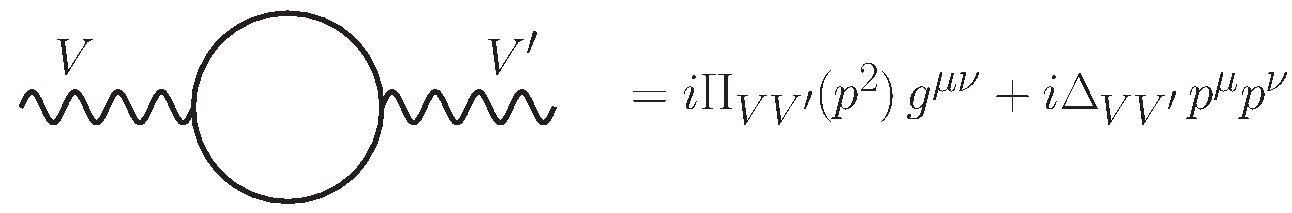
\includegraphics[scale=0.5]{fig1.pdf}
\end{center}
\caption{Gauge boson two-point  functions.}
\label{fig:STU-propagator}
\end{figure}
%%%%%%%%%%%%%%%%%%%%%%%%%%%%%%%%%%%%%%%%%%%%%%%%%%%%%%%%%%%%%%%%%
The SDFM model presents new contributions to the electroweak precision observables (EWPO). 
The ($V = W,\gamma, Z$) gauge bosons  two-point functions shown in Fig.~\ref{fig:STU-propagator} are modified by the presence of the new $Z_2$-odd particles circulating in the loop. 
It gives a new contribution to the Peskin-Takeuchi $S$, $T$, $U$ parameters~\cite{PhysRevD.46.381}, which are defined as
%
\begin{align}
\label{eq:ST-definition}
S=&\dfrac{4s^2c^2}{\alpha}\left(\dfrac{\Pi_{ZZ}(m_Z^2)
-\Pi_{ZZ}(0)}{m_Z^2}-\dfrac{c^2-s^2}{sc}\dfrac{\Pi_{Z\gamma}(m_Z^2)}{m_Z^2}
-\dfrac{\Pi_{\gamma\gamma}(m_Z^2)}{m_Z^2}\right)\\
T=&\dfrac{1}{\alpha}\left(\dfrac{\Pi_{WW}(0)}{m_W^2}-\dfrac{\Pi_{ZZ}(0)}{m_Z^2}\right)\\
U=&\dfrac{4 s^2}{\alpha}\left(\Pi'_{WW}(0)-c^2\,\Pi'_{ZZ}(0)-2\,sc\,\Pi'_{Z\gamma}(0)-s^2\Pi'_{\gamma\gamma}(0)\right) \,,
\end{align}
with $s=\sin\theta_W$ and $c=\cos\theta_W$ \footnote{The definition for the $\Pi$ functions can be found in the Refs.~\cite{Abe:2014gua} and \cite{D'Eramo:2007ga}.}.  
%
Actually, the only important parameters are $S$ and $T$. The $U$ parameter is not useful in practice because its contribution from most new physics models is very small. It can be shown that $U$ actually parametrizes the coefficient of a dimension-eight operator, while $S$ and $T$ can be represented as a dimension-six operator. 
%
Something important is that a charge conjugation symmetry ($\tilde{R}_u\leftrightarrow R_d$) in the Lagrangian~\eqref{eq:lt13A} 
is obtained when $\lambda_u=|\lambda_d|$ and this causes a vanishing DM coupling with the $Z$ gauge boson ($N_{21}=N_{31}$ in the Eq.\eqref{eq:cZXiXj}). Even more, due to this custodial symmetry, the new contribution to the $T$ parameter vanishes for this particular case. 

For the analysis carried out in this work, it has been used the correction $\Delta S$ and $\Delta T$  reported in the Ref.~\cite{D'Eramo:2007ga}~\footnote{ A crosscheck has been done with the Ref.~\cite{Abe:2014gua}.}. 
Those are given by
%
\begin{eqnarray}
\Delta T & = & \sum_{i=1}^{3}\left[
\left(V_{1i}\right)^{2}\widetilde{A}\left(M,m_{i}\right)+
\left(V_{2i}\right)^{2}\widetilde{A}\left(M,-m_{i}\right)\right]
\nonumber\\ & & -\frac{1}{2}\sum_{i,j=1}^{3}
\left(V_{1i}V_{2j}+V_{2i}V_{1j}\right)^{2}\widetilde{A}\left(m_{i},-m_{j}\right) \,,
\end{eqnarray}
%
\begin{equation}
\Delta S =   \frac{1}{2}\sum_{i,j=1}^{3}
\left(V_{1i}V_{2j}+V_{2i}V_{1j}\right)^{2}\widetilde{F}\left(m_{i},-m_{j}\right)-\widetilde{F}\left(\mu,\mu\right) \,,
\end{equation}
where
\begin{equation}
\widetilde{A}\left(m_{1},m_{2}\right)\equiv
\frac{1}{2\alpha_{em}v^{2}}\Pi\left(0\right) \,,
\end{equation}
%
\begin{equation}
\widetilde{F}\left(m_{1},m_{2}\right)\equiv 4\pi
\Pi^{'}\left(0\right) \,,
\end{equation}
%
\begin{eqnarray}
\Pi(0) & = & \frac{1}{16\pi^{2}}\left[
\left(m_{1}-m_{2}\right)^{2}\ln\frac{\Lambda^{4}}{m_{1}^{2}m_{2}^{2}}-2m_{1}m_{2}\right.
\nonumber\\ & &
+\left.\frac{2m_{1}m_{2}\left(m_{1}^{2}+m_{2}^{2}\right)-m_{1}^{4}-m_{2}^{4}}{m_{1}^{2}-m_{2}^{2}}
\ln\frac{m_{1}^{2}}{m_{2}^{2}}\right] \,,
\end{eqnarray}
%
\begin{eqnarray}
\Pi^{'}(0) & = & \frac{1}{24\pi^{2}}\left[
-\ln\frac{\Lambda^{4}}{m_{1}^{2}m_{2}^{2}}-
\frac{m_{1}m_{2}\left(3m_{1}^{2}-4m_{1}m_{2}+3m_{2}^{2}\right)}{\left(m_{1}^{2}-m_{2}^{2}\right)^{2}}\right.
{}\nonumber\\ & &
{}+\left.\frac{m_{1}^{6}+m_{2}^{6}-3m_{1}^{2}m_{2}^{2}\left(m_{1}^{2}+m_{2}^{2}\right)+6m_{1}^{3}m_{2}^{3}}
{\left(m_{1}^{2}-m_{2}^{2}\right)^{3}}\ln\frac{m_{1}^{2}}{m_{2}^{2}}\right] \,.
\end{eqnarray}
%
These expressions are valid for Dirac particles and for Majorana fermions with an extra factor of two and with $\Lambda$ the cutoff of the loop integral which
disappears at the end of the computation.

To be compatible with the parametrization used in the Eq.~\eqref{eq:Mchis}, the next identification was carry out: $M\to -M_D$ , $\mu\to -2M_N$ , $\alpha=\frac{\lambda_u+\lambda_d}{2}$ , $\beta'=\frac{\lambda_u-\lambda_d}{2}$ and the $V_{ij}$ coefficients were obtained after the diagonalization of the matrix
%
\begin{equation}
 \mathbf{M}^{\chi}=\left(
\begin{array}{ccc}
M & 0 & -\beta' v \\
0 & -M & -\alpha v\\
-\beta' v & -\alpha v & -2 \mu
\end{array} \right) \,,
\end{equation}
which is the neutral fermion mass matrix obtained in the basis used in the Ref.~\cite{D'Eramo:2007ga}.

%
%%%%%%%%%%%%%%%%%%%%%%%%%%% PLOT EDM   %%%%%%%%%%%%%%%%%%%%%%%%%%%
\begin{figure}[h]
\begin{center}
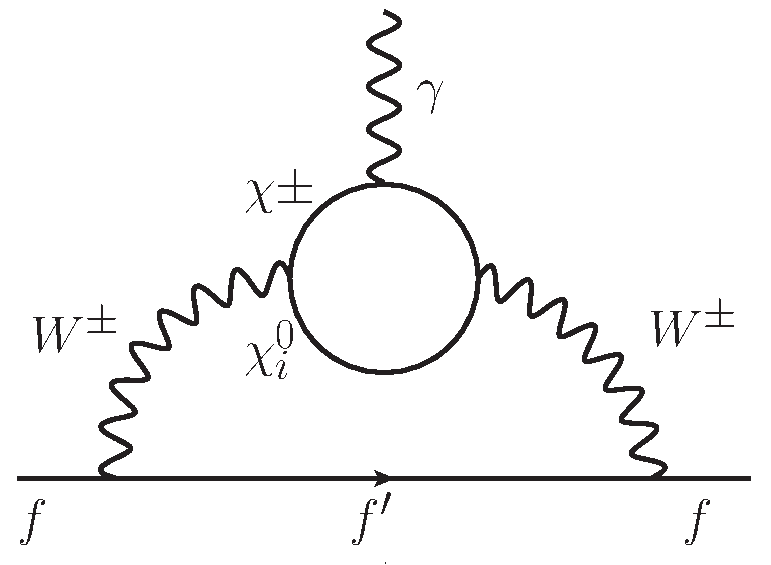
\includegraphics[scale=0.4]{fig2.pdf}
\end{center}
\caption{Contribution to the electric dipole moment (EDM) of a fermions $f$ in the SM.}
\label{fig:EDM}
\end{figure}
%%%%%%%%%%%%%%%%%%%%%%%%%%%%%%%%%%%%%%%%%%%%%%%%%%%%%%%%%%%%%%%%%
%

As a final comment, the contributions to the electric dipole moment (EDM) of the particles in the SM, which is the process shown in Fig.~\ref{fig:EDM}
happens when the Yukawa couplings $\lambda_u , \lambda_d$ are complex numbers. However, this work is not focused on that direction because the couplings were chosen as real numbers. Those issues were discussed in the Ref.~\cite{Abe:2014gua}.










%%%%%%%%%%%%%%%%%%%%%%%%%%%%%%%%%%%%%%%%%%%%%%%%%%%%%%%%%%%%%%%%%%%%%%%%%%%%%%
\section{The dark matter abundance $\Omega h^2$ }
\label{sec:abundance}
%
%%%%%%%%%%%%%%%%%%%%%%%% PLOT Fig8. %%%%%%%%%%%%%%%%%%%%%%%%%%%
\begin{figure}[h]
\begin{center}
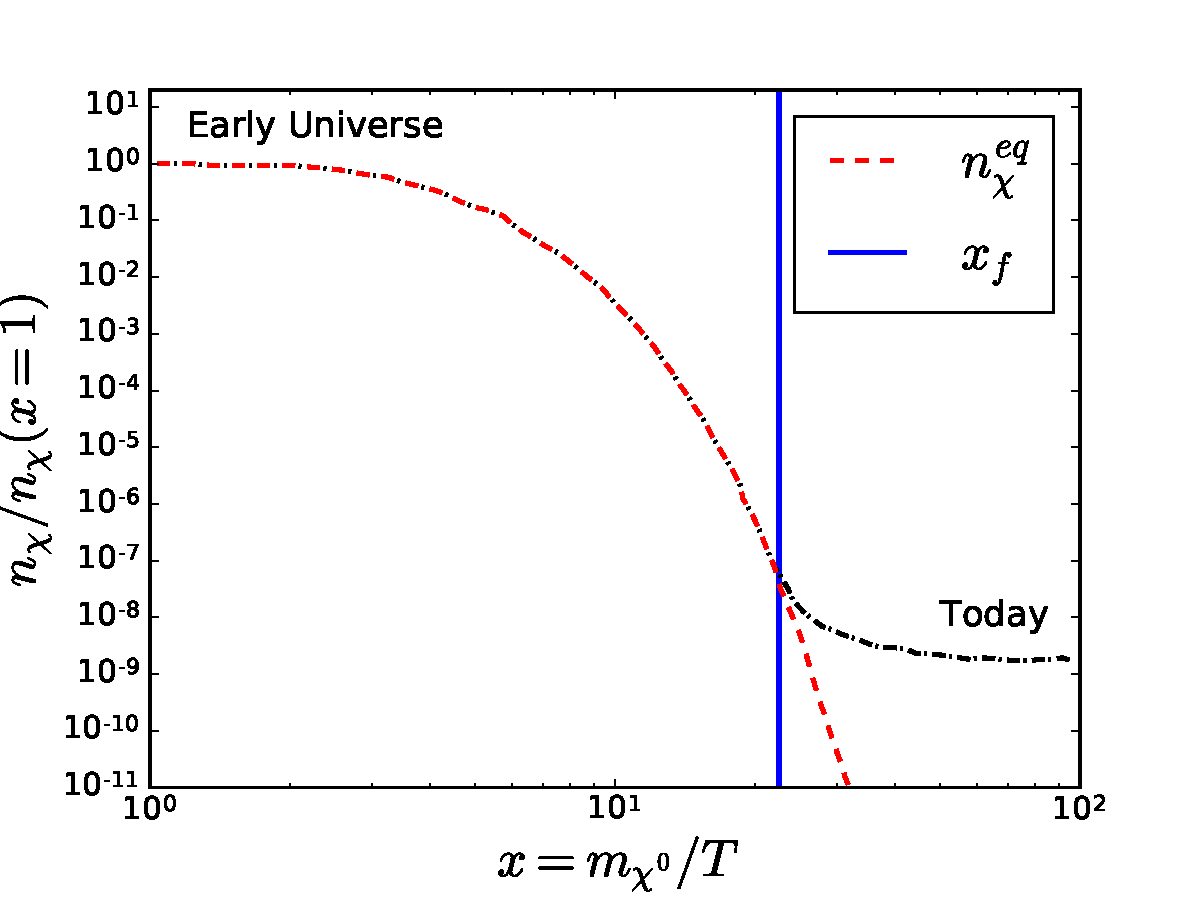
\includegraphics[scale=0.45]{freeze-out.pdf}
\end{center}
\caption{A DM number density illustration which follows the equilibrium density ($n_{\chi}^{\text{eq}}$) to the point $x_f$ (``freeze-out"). After that it remains constant to today.}
\label{fig:freeze-out}
\end{figure}
%%%%%%%%%%%%%%%%%%%%%%%%%%%%%%%%%%%%%%%%%%%%%%%%%%%%%%%%%%%%%%%%%
%
The DM abundance for the SDFDM model can be computed using the standard analysis for a cold relic density decoupled in the early Universe. In this picture, the evolution of the number density of the DM particles $n_{\chi}$ is governed by the Boltzmann equation~\cite{Kolb:1990vq}
\begin{align}
\dfrac{dn_{\chi}}{dt}+3Hn_{\chi}=&-\langle \sigma v \rangle \left[n_{\chi}^2-(n_{\chi}^{\text{eq}})^2\right]\,,
\end{align}
where $H$ is the Hubble parameter that characterize the Universe's expansion, $n_{\chi}^{\text{eq}}$ is the number density when the DM particles are in equilibrium, i.e. when the DM particles are not decoupled in the early Universe and $\langle \sigma v \rangle$ is the thermal velocity averaged self-annihilation cross section.

The Boltzmann equation can be solved approximately when
the temperature dependence of the  $\langle \sigma v \rangle$ is parameterized as
%
\begin{align}
\langle\sigma v\rangle= &\, \sigma_0\, x^{-n}\,,
\end{align} 
%
where $\sigma_0$ is the cross section to zero temperature, $x=m_{\chi^0}/T$ and $n=0$ corresponds to the s-wave  contribution, $n=1$ to the p-wave, etc.

The idea of the concept of the relic density is shown in Fig.~\ref{fig:freeze-out}. In the early Universe the DM number density $n_{\chi}$ is approximately given by $n_{\chi}^{\text{eq}}$.
However, with the expansion of the Universe, the temperature drops below the mass of the DM particle and the reaction rate $\Gamma(\chi^0\chi^0\leftrightarrow \text{SM\, SM})$ gets slower than the expansion of the Universe and the $n_{\chi}^{\text{eq}}$ drops exponentially until a point called ``freeze-out" ($x_f=m_{\chi^0}/T_f$).
In this point, the reaction is not fast enough to hold the equilibrium and the DM particle is decoupled of the SM particles and its density remains constant to today.  
In general, the Boltzmann equation can be solved  before the ``freeze-out" when $n_{\chi}\approx n_{\chi}^{\text{eq}}$ and  after that,  when $n_{\chi}^{\text{eq}} \ll n_{\chi}$ and $n_{\chi}^{\text{eq}}$ can be neglected.
The complete solution is obtained by using the matching between last two solutions just at the `freeze-out" point.
Without entering in more details, this solution is given by~\cite{D'Eramo:2007ga}
%
\begin{align}
\Omega h^2  \approx & (n+1)\dfrac{x_f}{g_*^{1/2}}\dfrac{0.034\, \text{pb}}{\langle \sigma v_r\rangle} \,,
\end{align} 
where the variable $x_f$ at the ``freeze-out" is computed solving the equation
\begin{align}
x_f+(n+1)\log x_f \approx \log\left[0.038\left(n+1\right)\left(\dfrac{g}{g_*^{1/2}}\right)M_{p}\,m_{\chi^0}\,\sigma_{0}\right]\,,
\end{align} 
with $M_{p}=1.22 \times 10^{19}$ GeV the Planck mass.

These expressions were computed and checked using \textsc{micrOMEGAs 4.1.8}~\cite{Belanger:2014vza}. A good agreement was obtained for some special cases of the parameter space where the $\langle \sigma v \rangle$ is easily computed by hand. However, the numerical solution obtained with \textsc{micrOMEGAs} was used because it takes care of the complete $\langle \sigma v \rangle$ when the self-annihilation of DM takes place in all the possible final channels that will be described later. Even more,  \textsc{micrOMEGAs} takes care of difficult regions of the parameter space, for instance, the process of coannihilations and resonances~\cite{Griest:1990kh}. 












%%%%%%%%%%%%%%%%%%%%%%%%%%%%%%%%%%%%%%%%%%%%%%%%%%%%%%%%%%%%%%%%%%%%%%%%%%%%%%%%%%%%%%%%%%%%%%%%%%%%%%%%%%%%
\section{Model's implementation}
%
%%%%%%%%%%%%%%%%%%%%%%%% PLOT Fig8. %%%%%%%%%%%%%%%%%%%%%%%%%%%
\begin{figure}[h]
\begin{center}
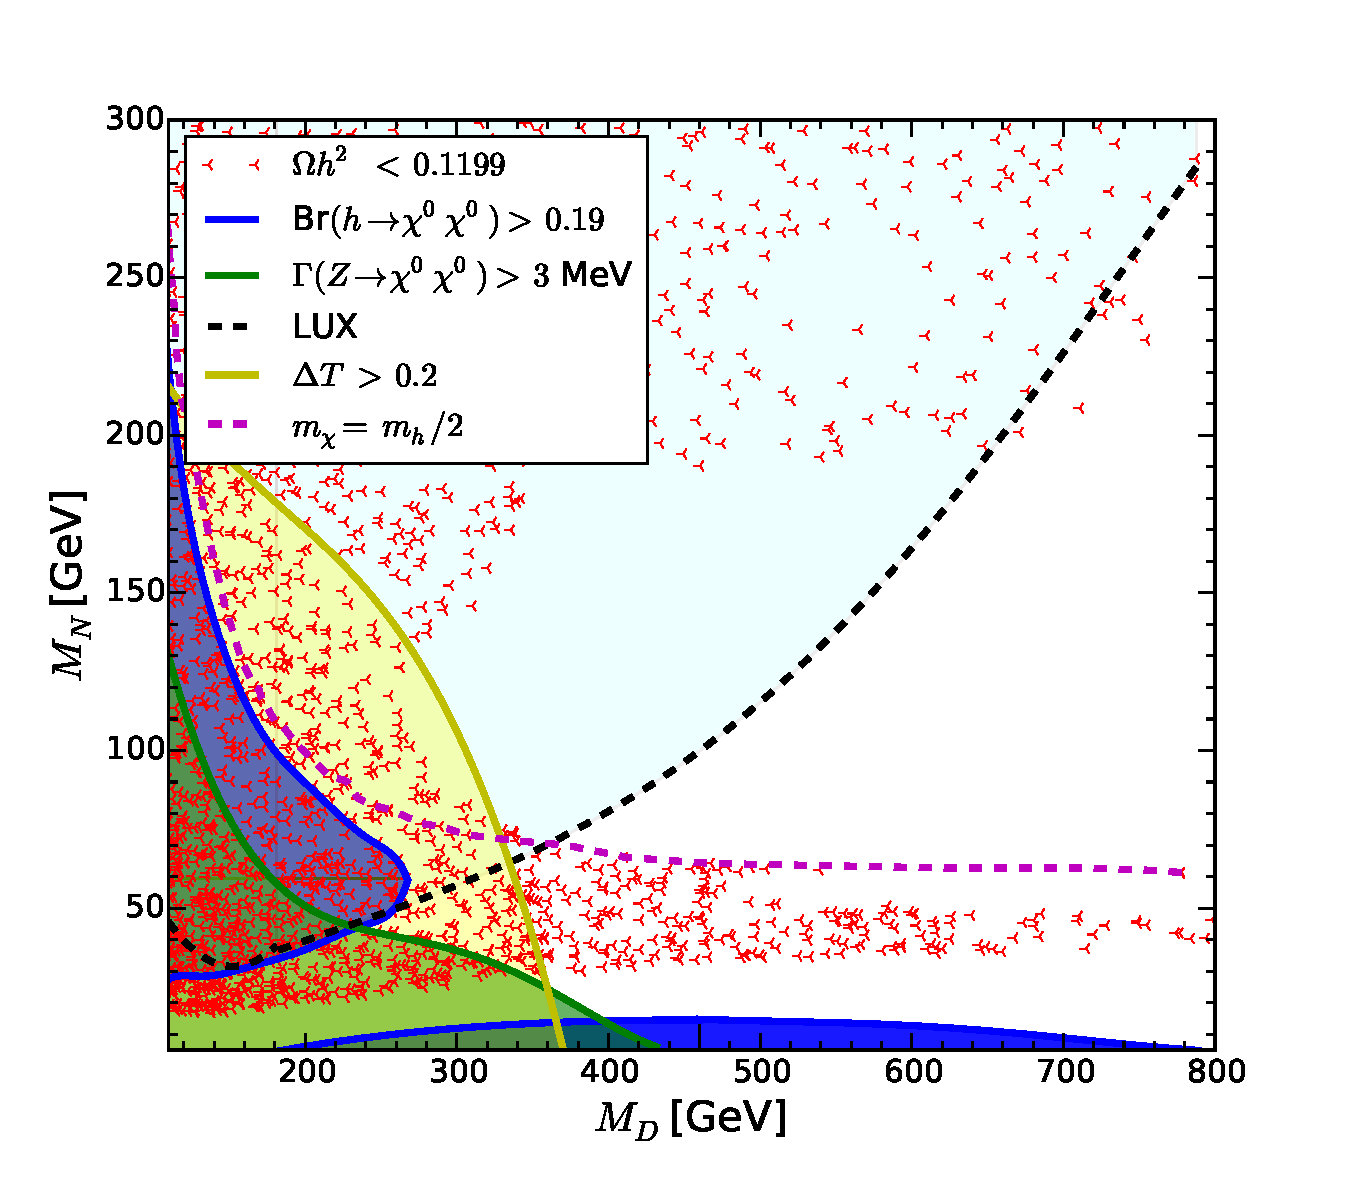
\includegraphics[scale=0.5]{fig8.pdf}
\end{center}
\caption{Constraints on the SDFDM model in the low mass region for $\lambda=1$ and $\tan\beta=-20$. Above the black dashed line: region exclude by LUX ($\sigma_{SI}$). Yellow: region excluded by EWPO. Green (Blue): region excluded by the $Z$ ($h$) invisible decay. The magenta dashed line corresponds to $m_{\chi^0}=m_h/2 $.}
\label{fig:fig8-1505.03867}
\end{figure}
%%%%%%%%%%%%%%%%%%%%%%%%%%%%%%%%%%%%%%%%%%%%%%%%%%%%%%%%%%%%%%%%%

The SDFDM model was implemented in \textsc{Feynrules 2.3}~\cite{Christensen:2008py} and a crosscheck was done using the \texttt{BSM-Toolbox}~\cite{Staub:2011dp} of \texttt{SARAH}~\cite{Staub:2008uz,Staub:2013tta}.
%
The first step was to reproduce some of the known results for this model. 
For that purpose, a benchmark point was taken in order to check the implementation.
For instance, Fig.8 of the Ref.~\cite{Calibbi:2015nha} that shows the behavior of the model for the specific case of $\lambda=1$ and $\tan\beta=-20$.
% 
We used the LUX-2013~\cite{Akerib:2013tjd}  limits for spin-independent cross section with nucleons
and we assumed that the DM  relic density saturates the Planck measurement $\Omega h^2=(0.1199 \pm 0.0027)$~\cite{Ade:2013zuv} at the $3\,\sigma$. 
The results are shown in Fig.~\ref{fig:fig8-1505.03867}.
There, the region above the black dashed line is excluded by LUX. In the same way, the green (blue) region is excluded by the $Z$ ($H$) invisible decay and the yellow region  is excluded by the correction to the EWPO parameters (we disagree with the Ref.~\cite{Calibbi:2015nha} by a factor two in the $\Delta T$ computation,
that factor takes into account that DM particles are Majorana fermions).
Note that the boundary of the region given by the red points reproduces the experimental value of  $\Omega h^2$, while the remaining white zones have an overabundance of the DM relic density.



 






%%%%%%%%%%%%%%%%%%%%%%%%%%%%%%%%%%%%%%%%%%%%%%%%%%%%%%%%%%%%%%%%%%%%%%%%%%%%%%
\section{Indirect detection }
\label{sec:indirec-detection}

%\subsection{DM self-annihilation channels}

\begin{figure}
\begin{center}
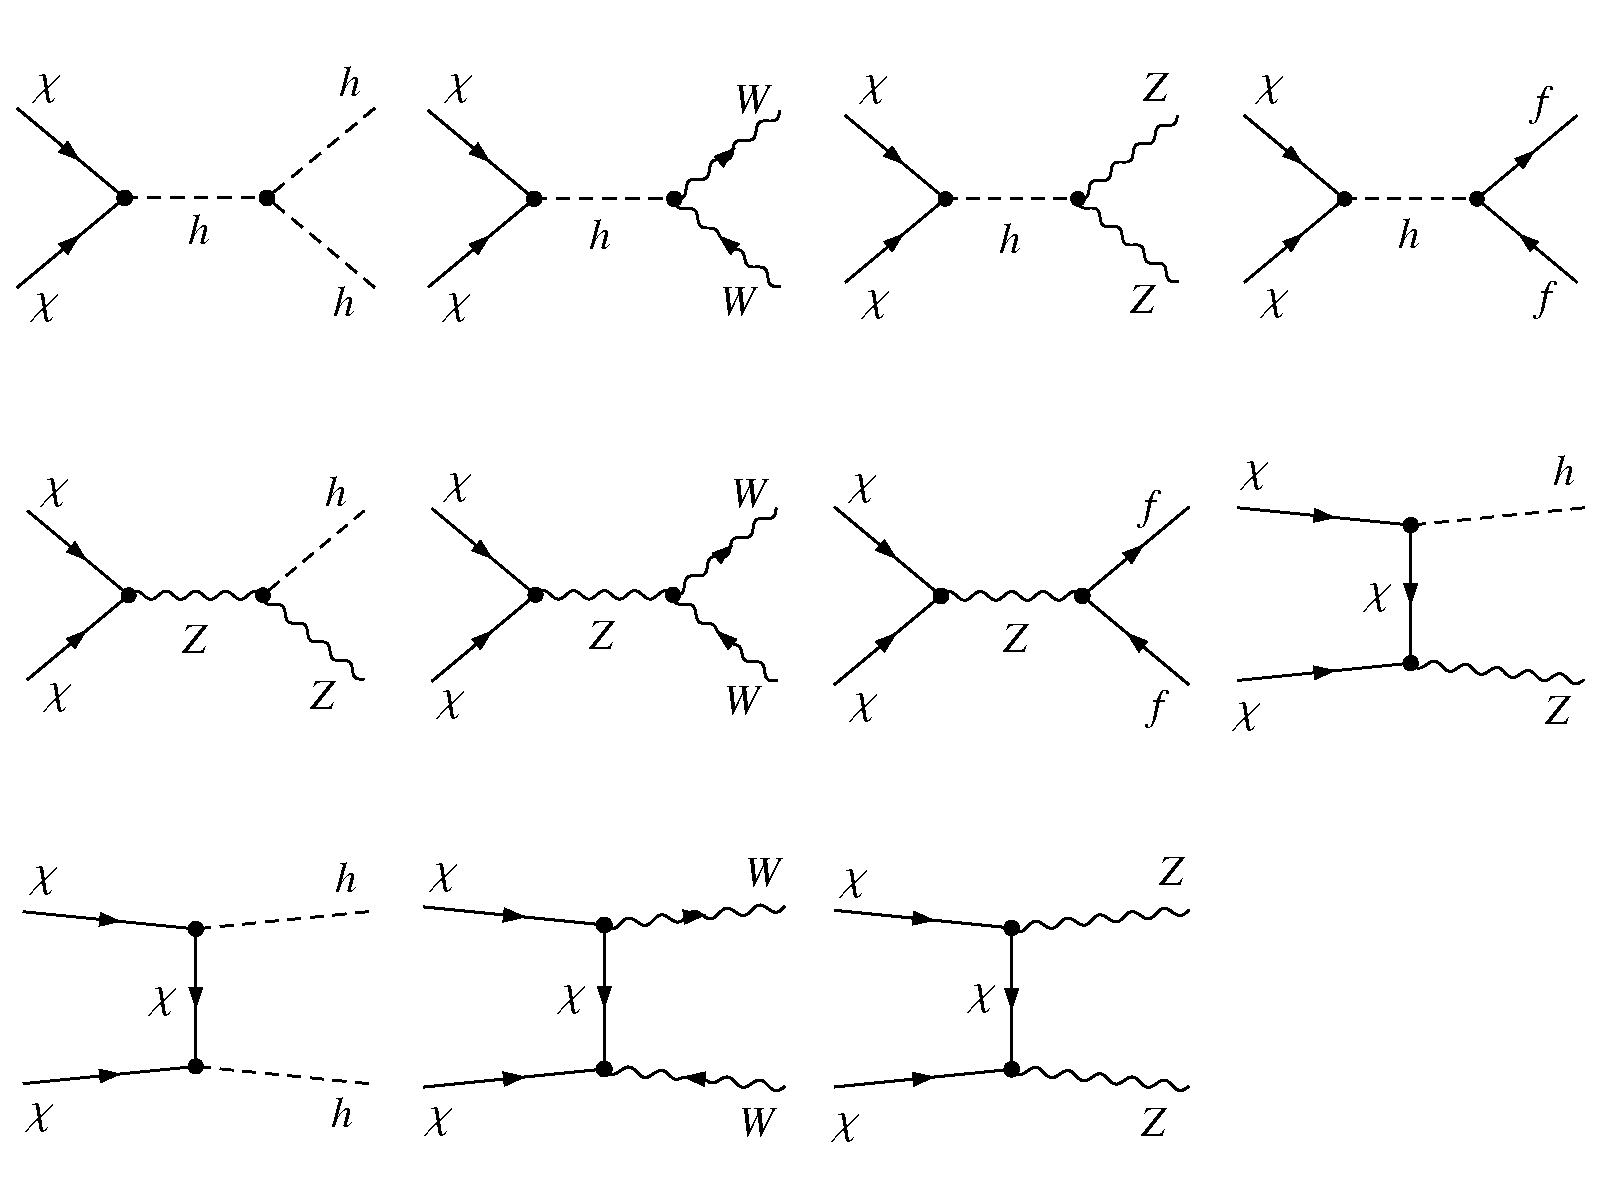
\includegraphics[scale=0.47]{XXtoSM}
\end{center}
\caption{Self-annihilation channels a tree level in the SDFDM model. The u-channels are not shown. They were generated using \textsc{FeynArts}~\cite{Hahn:2000kx}.}
\label{fig:self-channels}
\end{figure}

At tree level, the interaction between the DM and the SM sector is mediated by the $W$, $Z$ and $H$ gauge bosons.
In this model, DM particle ($\chi^0$) can self-annihilate into $\bar{f}f$, $ZZ$, $W^+W^-$ and $hh$ final states through  $s$-channel Higgs and $Z$ boson exchange and into $ZZ$, $W^+W^-$ states via $t$-channel $\chi_i^0$ and $\chi^{\pm}$ exchange. Annihilation into a mixture of weak gauge bosons $Zh$ is also possible through the exchange of a $\chi_i\neq\chi^0$  in the $t$-channel or a $Z$ in the $s$-channel. Those annihilation channels are shown in Fig.~\ref{fig:self-channels}.  We remark in passing that gamma-ray lines $\gamma\gamma$ and $\gamma Z$ can also be produced at one-loop level.
Of particular importance for indirect detection studies in this framework is the fact that since DM annihilations into fermion pairs mediated by the Higgs are $p$-wave suppressed and there is not $s$-wave amplitude, the annihilations produced through the $Z$ exchange are dominant. We note that the later is also helicity suppressed, which implies that the main annihilation channel is the $t\bar{t}$ ($b\bar{b}$) for a dark matter mass above (below) the top mass, with $\langle\sigma v \rangle\lesssim 10^{-27}$ cm$^3$ s$^{-1}$ for $m_{\chi^0}<m_W$ \cite{Calibbi:2015nha}. 

In the case of DM particles going into gauge bosons, only those processes in the $t$-channel are relevant because they do not suffer velocity suppression. Such a non-velocity suppression is also present in $s$ and $t$ channels for the annihilation into $Zh$. 
In contrast, processes in which DM self-annihilates into Higgs bosons are velocity suppressed. 










\subsection{Scanning and constraints}
\label{sec:Parameter-scan}

In order to see the behavior of the DM observables in this model, the parameter space was scanned considering the following ranges of model parameters   
\begin{align}\label{eq:scan}
100<M_D/\text{GeV}<1000 \,, &\hspace{1cm}10 <M_N/\text{GeV}<1000\,,\nonumber\\
10^{-4}<\lambda<10 \,,&\hspace{1cm} 1\leq\left|\tan\beta\right|<60\,.
\end{align}
%
Essentially, we throw darts into this large space, generating several million random model points, and for each generated point we computed the DM relic density and the direct and indirect DM observables using \textsc{micrOMEGAs 4.1.8}~\cite{Belanger:2014vza} through \textsc{Feynrules 2.3}~\cite{Christensen:2008py}. Each individual model is then subjected to a large set of dark matter, precision measurement, and collider constraints. 
In particular, we assume that the DM  relic density saturates the Planck measurement $\Omega h^2=(0.1199 \pm 0.0027)$~\cite{Ade:2013zuv} at the $3\,\sigma$ level as we are interested in considering the case where this model accounts for the majority of DM. The model points are also required to be compatible with \textit{Fermi}-LAT \footnote{\textit{Fermi}  Large Area Telescope: \url{http://fermi.gsfc.nasa.gov/}.} constraints coming from dwarf spheroidal galaxies~\cite{Ackermann:2015zua}, as well as LUX~\cite{Akerib:2013tjd}, IceCube~\cite{2013PhRvL.110m1302A}, PICO-2L~\cite{Amole:2016pye} and PICO-60~\cite{Amole:2015pla}  limits for spin-independent and spin-dependent detection studies. 
Since the SDFM model presents new contributions to the EW precision observables (EWPO) as was described in the section~\ref{sec:EWPO}, we impose the condition that $\Delta T < 0.2$ given that the contribution to $S$ is always negligible \cite{Calibbi:2015nha}.  Finally, the limit obtained from searches of charged vector-like particles by LEP~\cite{ALEPH:2005ab} has been taken into account by imposing the condition $M_D > 100$~GeV in Eq.~\eqref{eq:scan}. 

%%%%%%%%%%%%%%%%%%%%%%%% PLOT SV %%%%%%%%%%%%%%%%%%%%%%%%%%%
\begin{figure}[h]
\begin{center}
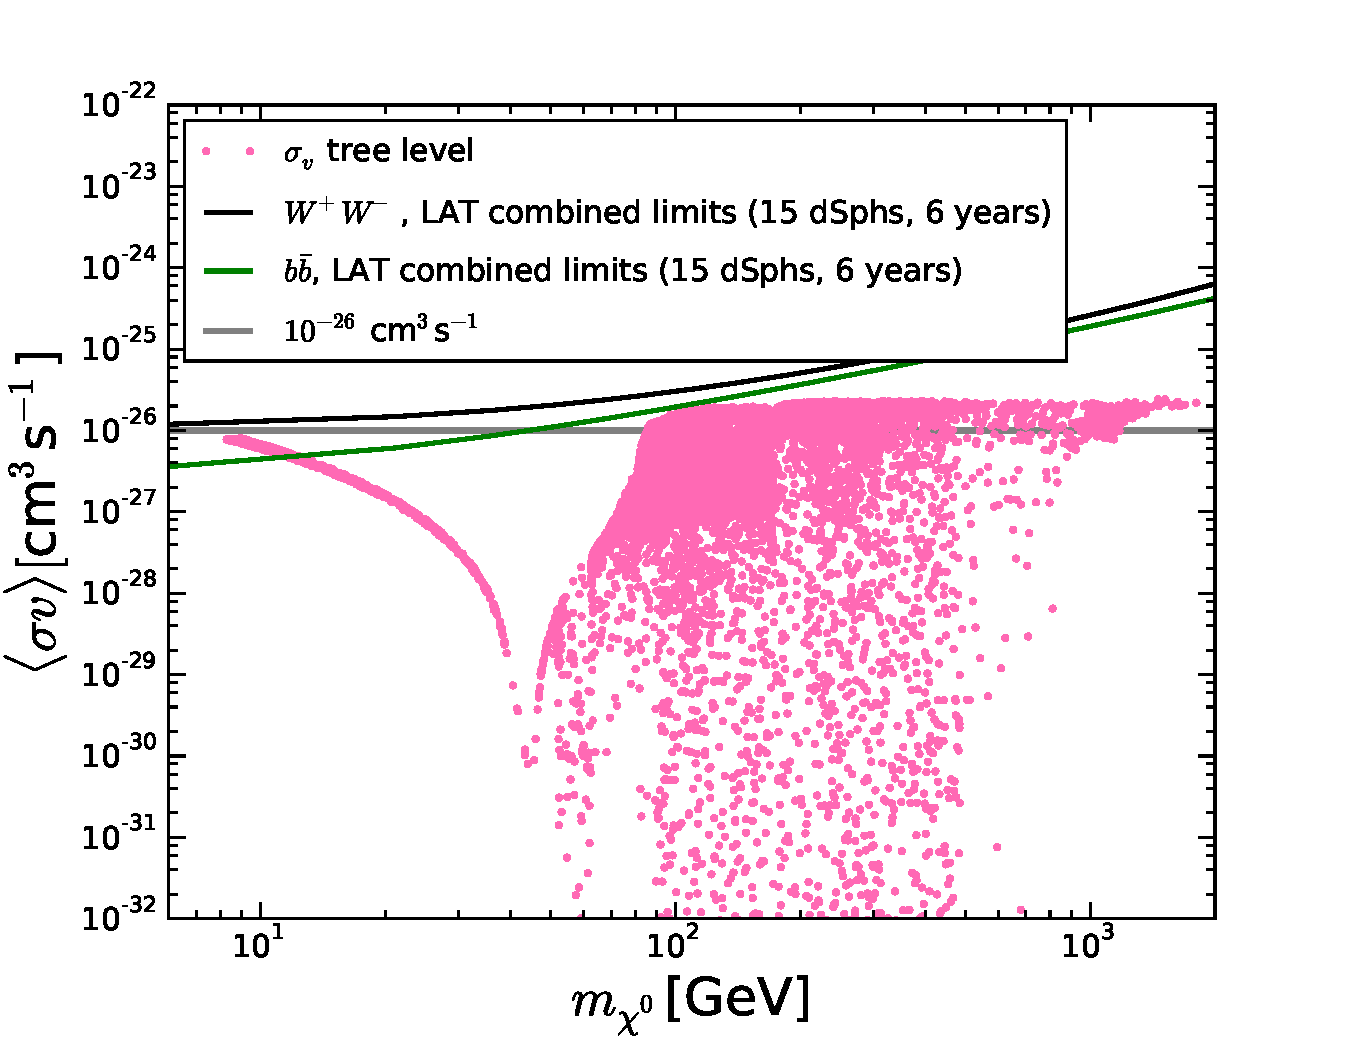
\includegraphics[scale=0.45]{sigmav-T13A}
\end{center}
\caption{Velocity average annihilation cross-section $\langle\sigma v\rangle$, generated randomly for a big sample of the parameters of the SDFDM model that take into account the correct relic density (see section~\ref{sec:Parameter-scan}). The green (black) line is the current constraint of indirect detection for DM self-annihilation into $b\bar{b}$ ($W^+W^-$) in the dwarf spheroidal galaxies (dSph) at 95$\%$ C.L~\cite{Ackermann:2015zua}. The gray line represents the prediction of the WIMP paradigm where the $\langle\sigma v\rangle$ reach the thermal value $10^{-26}\text{cm}^{3}\text{s}^{-1}$.}
\label{fig:sigmav-random}
\end{figure}
%%%%%%%%%%%%%%%%%%%%%%%%%%%%%%%%%%%%%%%%%%%%%%%%%%%%%%%%%%%%%%%%%

In Fig.~\ref{fig:sigmav-random}, it is shown the total velocity average annihilation cross-section $\langle\sigma v\rangle$ for the DM self-annihilation into SM particles including two and three final states.
%
Also, it is shown the current and strongest \textit{Fermi}  Large Area Telescope (LAT)
constraints of DM self-annihilation into $b\bar{b}$ quarks and $W^+W^-$ gauge bosons in the dwarf spheroidal galaxies (dSph). It can be seen that indirect detection does not put strong constraints on the parameter space of the SDFDM model. All the models are alive with the current indirect detection constraints.    









%%%%%%%%%%%%%%%%%%%%%%%%%%%%%%%%%%%%%%%%%%%%%%%%%%%%%%%%%%%%%%%%%%%%%
\section{Direct detection}
Regarding direct detection, the Higgs $h$ ($Z$ gauge bosson) exchanging leads to spin-independent (spin-dependent) DM nucleon scattering (see Fig.~\ref{fig:SD_SI}). From Eq.~\eqref{eq:cZXX} is clear that the spin-dependent (SD) cross section vanishes for $\cos2\beta=0$ or $|m_{\chi^0}|=M_D$, implying for both cases that $\tan\beta=\pm 1$. In the same vein, from Eq.~\eqref{eq:cHXX} the spin-independent (SI) cross section vanishes (i.e. a blind spot as discussed by Ref.~\cite{Cheung:2013dua}) for $\sin2\beta=-m_{\chi^0}/M_D$, which using the characteristic equation of the Appendix~\eqref{sec:analyt-form-mass}
leads to $m_{\chi^0}=M_N, M_D$. Note that $\sigma_{SI}=0$ if $\tan\beta<0$ and only if $M_N>M_D$, both $\sigma_{SI}$ and $\sigma_{SD}$ can be zero simultaneously. 
%
\begin{figure}[h]
  \centering
  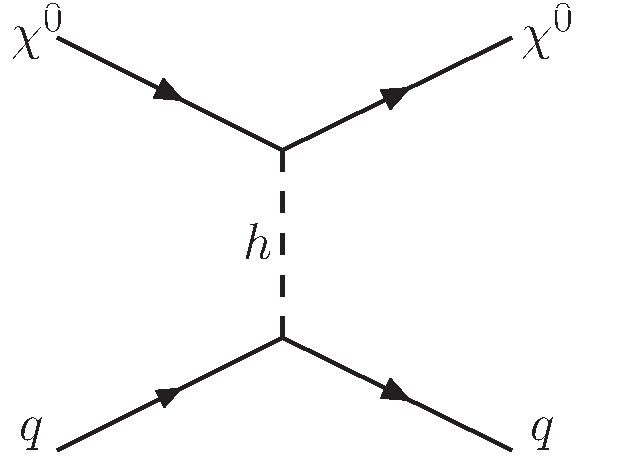
\includegraphics[scale=0.4]{SI} 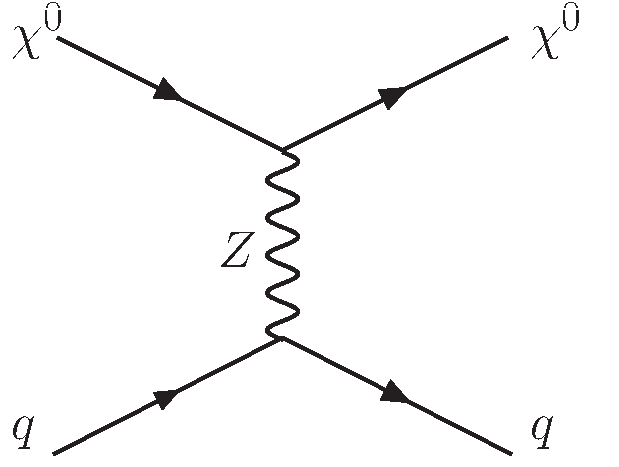
\includegraphics[scale=0.4]{SD}
  \caption{DM inelastic scattering with the quarks that compose the nucleons (protons and neutrons).}
  \label{fig:SD_SI}
\end{figure}









%%%%%%%%%%%%%%%%%%%%%%%%%%%%%%%%%%%%%%%%%%%%%%%%%%%%%%%%%%%%%%%%%%%%%%%%%%%%%%%%%%%%%%%%%%%%%%%%%%%%
\subsection{The spin-independent cross section $\sigma_{SI}$}
%
The DM scattering with the nucleons $N$ (protons and neutrons) is an effective interaction because nucleons are made of quarks. When the mediator is the Higgs gauge boson, the scalar interaction is spin-independent. In order to compute this scattering is reasonable to think in the next effective interaction
%  
\begin{align}
\mathcal{L}_{\text{SM}}\supset \sum_{q}\dfrac{m_q}{v}h\bar{q}q
= & |N\rangle\langle N|\sum_{q}\dfrac{m_q}{v}h\bar{q}q |N\rangle\langle N|
=  \dfrac{h}{v}\langle N|\sum_{q}m_q\bar{q}q|N\rangle |N\rangle\langle N| \nonumber \\
= & \dfrac{m_Nf_N}{v}h\bar{N}N\,,
\end{align}
where $\langle N|\sum_{q}m_q\bar{q}q|N\rangle=m_Nf_N$ is a QCD form factor, which is experimentally determined~\cite{Belanger:2014vza}~\cite{Abdallah:2015ter}. Using this Lagrangian, it is possible to compute the spin-independent cross section (see the Appendix~\ref{sec:SI-amplitude}). It is given by
\begin{align}
\label{eq:SI-tree-level}
\sigma_{SI}=\dfrac{m_r^2}{\pi}\left(\dfrac{c_{hX_1X_1}}{vm_h^2}\right)^2f_N^2m_N^2\,,
\end{align}
%
where $m_r=\dfrac{m_Nm_{\chi^0}}{(m_N+m_{\chi^0})}$
is the reduced mass of the dark matter-nucleon system ($m_N\approx 0.939\, \text{GeV}$ for the neutron and $m_N\approx 0.938\, \text{GeV}$ for the proton). 

%%%%%%%%%%%%%%%%%%%%%%%%%%%%%%%%%%%% PLOT: SI %%%%%%%%
\begin{figure}[h]
\begin{center}
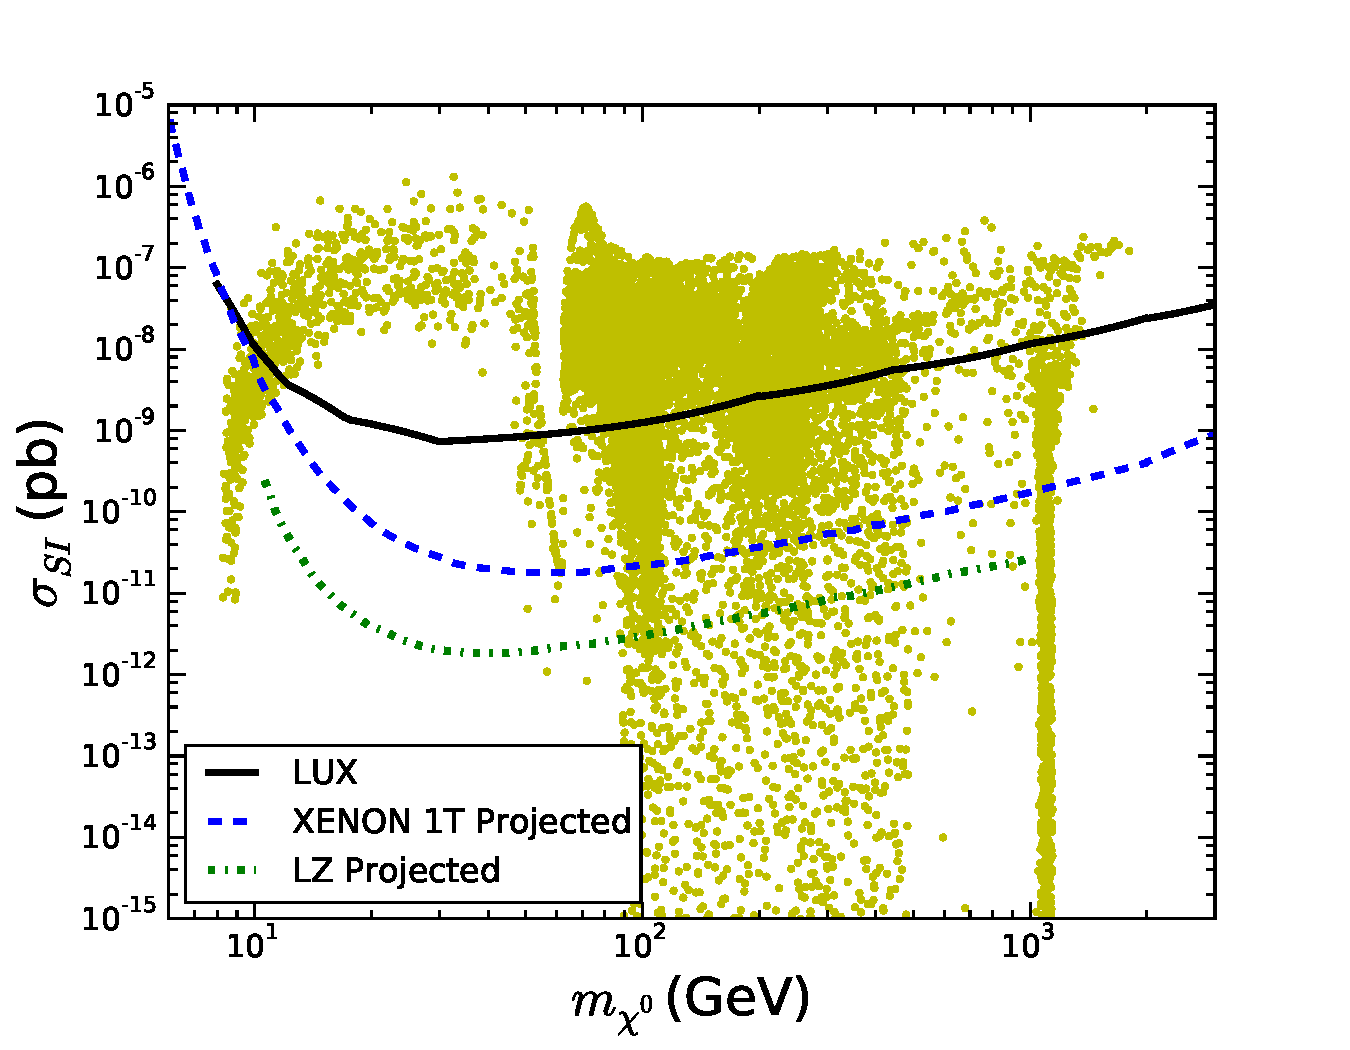
\includegraphics[scale=0.45]{sigmaSI-T13A}  
\caption{Spin-independent cross section in the SDFDM model in comparison to current and future direct detection limits. 
The panel displays current limits from the LUX experiment (black solid line)~\cite{2013arXiv1310.8214L} and the expected limits from the forthcoming XENON-1T and LZ~\cite{Cushman:2013zza} experiments (blue dashed and green dot-dashed lines).
}
\label{fig:sigma-SI}
\end{center}
\end{figure}
%%%%%%%%%%%%%%%%%%%%%%%%%%%%%%%%%%%%%%%%%%%%%%%%%%%%%%

In Fig.~\ref{fig:sigma-SI}, it is shown the spin-independent cross sections computed for a big sample of the parameters of the SDFDM model in Eq.~\eqref{eq:scan}. 
Also, it is shown the limits from the LUX-2013 experiment (black solid line)~\cite{2013arXiv1310.8214L} and the expected limits from the forthcoming XENON-1T and LZ~\cite{Cushman:2013zza} experiments (blue dashed and green dot-dashed lines).  
It can be seen that direct detection rules out some parameters space of this model. However, some of the models are alive with the current direct detection constraints.     








%%%%%%%%%%%%%%%%%%%%%%%%%%%%%%%%%%%%%%%%%%%%%%%%%%%%%%%%%%%%%%%%%%%%%%%%%%%%%%%%%%%%%%%%%%%%%%%%%%%%%%%%%%%
\subsection{The spin-dependent cross section $\sigma_{SD}$}

As it was said before, when the mediator in the scattering of the DM with nucleons $N$ (protons and neutrons) 
is the $Z$ gauge boson, the interaction is spin-dependent.
%
%%%%%%%%%%%%%%%%%%%%%%%%%%%%%%%%%%%% PLOT: SD  %%%%%%%%%%%
\begin{figure}[h]
\begin{center}
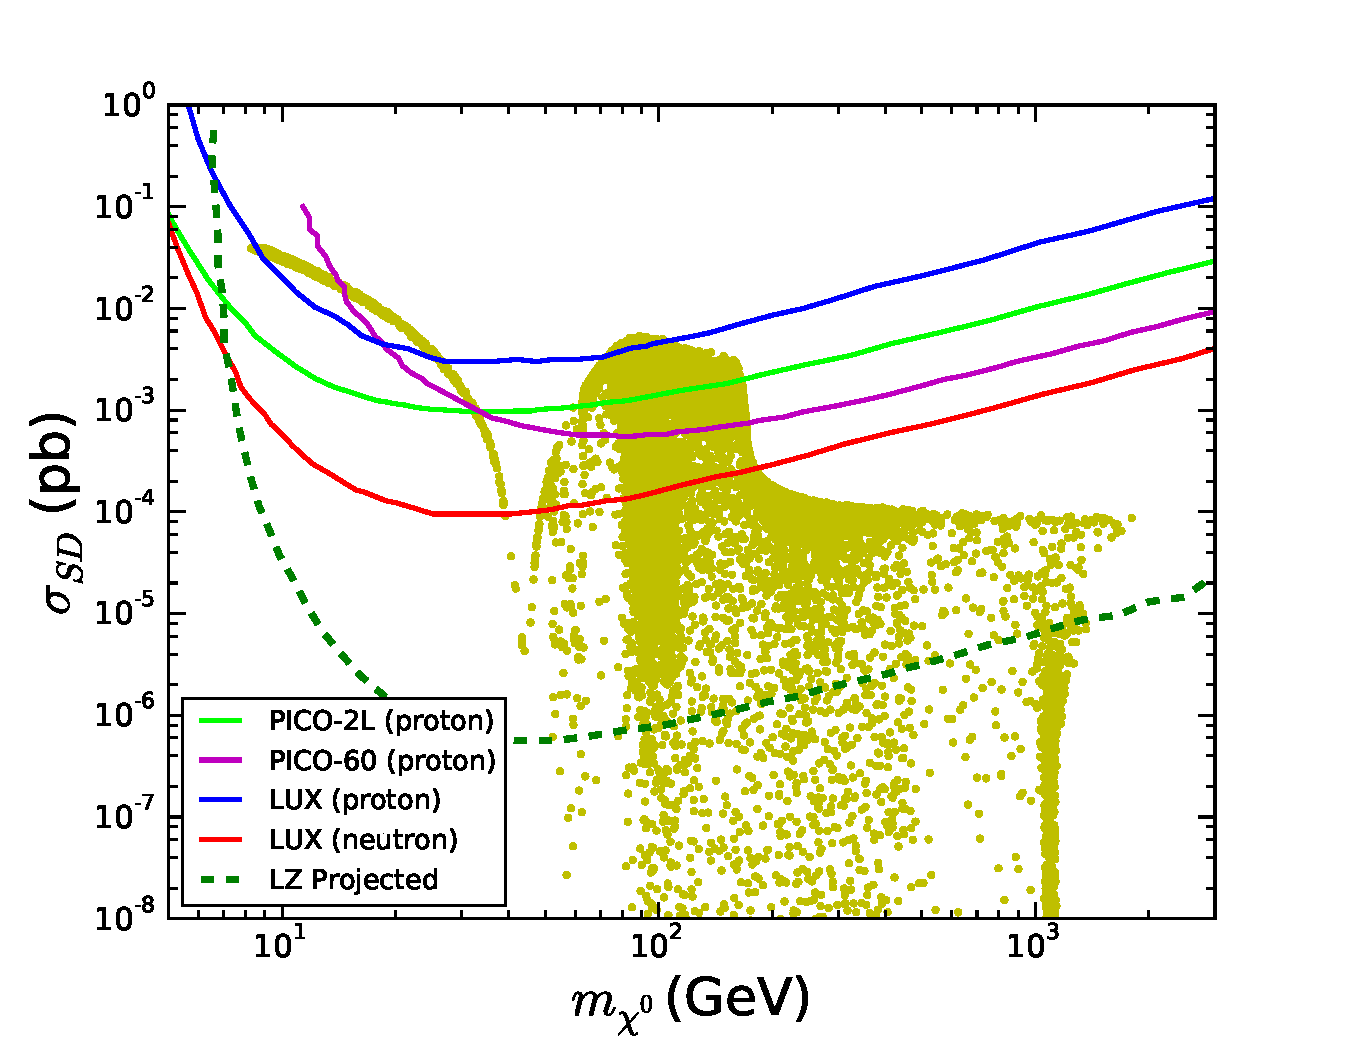
\includegraphics[scale=0.45]{sigmaSD-T13A} 
\caption{Spin-dependent cross section in the SDFDM model in comparison to current and future direct detection limits. 
The panel shows the PICO-2L~\cite{Amole:2016pye} (green light solid line) and PICO-60~\cite{Amole:2015pla} (magenta solid line) limits, as well as the LZ sensitivity (green dashed line). The most recent constraints from LUX~\cite{Akerib:2016lao} (red and blue solid lines) are also overlaid. 
}
\label{fig:sigma-SD}
\end{center}
\end{figure}
%%%%%%%%%%%%%%%%%%%%%%%%%%%%%%%%%%%%%%%%%%%%%%%%%%%%%%%%%%%%%%%
%
In Fig.~\ref{fig:sigma-SD}, it is shown the spin-dependent cross sections computed with \textsc{micrOMEGAs 4.1.8}~\cite{Belanger:2014vza} through \textsc{Feynrules 2.3}~\cite{Christensen:2008py}. Each individual model (point) saturates the Planck measurement value for the relic density $\Omega h^2=(0.1199\pm0.0027)$~\cite{Ade:2013zuv} at $3\sigma$ level. 
In Fig.~\ref{fig:sigma-SD}, it is also shown the PICO-2L~\cite{Amole:2016pye} (green light solid line) and PICO-60~\cite{Amole:2015pla} (magenta solid line) limits, as well as the LZ sensitivity (green dashed line). The most recent constraints from LUX-2016~\cite{Akerib:2016lao} (red and blue solid lines) are also overlaid. 
It can be seen that direct detection rules out some parameter space of this model. However, some of the models are alive with the current direct detection constraints, but in the future, the LZ experiment will rule out or confirm this model.

%CONECCTION
To finish this chapter, in the next section is described how to enlarge the SDFDM model in order to have masses for the active neutrinos of the SM.








%%%%%%%%%%%%%%%%%%%%%%%%%%%%%%%%%%%%%%%%%%%%%%%%%%%%%%%%%%%%%%%%%%%%%%%%%%%%%%%%%%%NEW
\section{Neutrino masses in the SDFDM model}
%
In view of the lack of signals of new physics in strong production at the
LHC, there is a growing interest in simplified models where the
production of new particles is only through electroweak processes,
with lesser constraints from LHC limits.
In particular, there are simple SM extensions with
dark matter candidates, such as the singlet scalar dark
matter (SSDM)
model~\cite{Silveira:1985rk,McDonald:1993ex,Burgess:2000yq}, or the
singlet-doublet fermion dark matter (SDFDM)
model~\cite{ArkaniHamed:2005yv,Mahbubani:2005pt,D'Eramo:2007ga,Enberg:2007rp,Cohen:2011ec,Cheung:2013dua}.
In this kind of models, the prospects for signals at LHC are in general
limited because of the softness of final SM particles coming from the
small charged to neutral mass gaps of the new particles, which is usually required 
to obtain the proper relic density.
In this sense, the addition of new particles motivated for example by
neutrino physics could open new detection possibilities, either
through new decay channels or additional mixings which increase the
mass gaps.

On those lines, scotogenic models~\cite{Ma:2006km}, featuring neutrino masses suppressed
by the same mechanism that stabilizes dark matter, have been thoroughly studied with specific predictions in almost all the current terrestrial and satellite detector experiments (For a review
see for example~\cite{Boucenna:2014zba}).
The simplest models correspond to extensions of the inert doublet
model~\cite{Deshpande:1977rw,Barbieri:2006dq} with extra singlet or
triplet fermions.
Recently, the full list of 35 scotogenic models with neutrino masses at
one-loop~\cite{Ma:1998dn,Bonnet:2012kz}~\footnote{The general
  realization of the Weinberg operator at two-loops have been undertaken
  in~\cite{Sierra:2014rxa}}, and at most triplet representations of
$SU(2)_L$, was presented in~\cite{Restrepo:2013aga} (and partially
in~\cite{Law:2013saa}).
The next to simplest scotogenic model is possibly the one where the
role of the singlet fermions is played by singlet scalars and the role
of the scalar inert doublet is played by a vector-like doublet fermion.
One additional singlet fermion is required to generate neutrino masses
at one-loop level.
This kind of extension of the singlet dark matter model is labeled
as the model T13A with $\alpha=0$ in \cite{Restrepo:2013aga}. The
extra fermion, required in order to have radiative neutrino masses, can
be the singlet in the SDFDM model.

In the simplest scotogenic model~\cite{Ma:2006km}, singlet fermion
dark matter is possible but quite restricted by lepton flavor
violation (LFV)~\cite{Toma:2013zsa,Vicente:2014wga}. 
In contrast, in the present model is shown that the region of the
parameter space, corresponding to fermion dark matter, is well below
the present and near future constraints on $\operatorname{Br}(\mu\to
e\gamma)$.

On the other hand, when the lightest $Z_2$-odd particle (LOP) is one
of the scalar singlets, in the regions of the parameter space 
compatible with constraints from LFV, the SDFDM model has promising signals at colliders,
thanks to the electroweak production of fermion doublets and possible
large branchings into charged leptons.

The dark matter phenomenology of both the SSDM and SDFDM models has
been extensively studied in the literature and recently
revisited in~\cite{Abe:2014gua}.
In this work both models will be joined and the possible effect of coannihilations with the
scalar singlets for fermion dark matter will be considered. 
We will see if these coannihilations tend to increase the relic
density of dark matter and if could modify the viable parameter space of
the SDFDM model. 








%%%%%%%%%%%%%%%%%%%%%%%%%%%%%%%%%%%%%%%%%%%%%%%%%%%%%%%%%%%%%%%%%%%%%%%%%%%%%%%%%%%%%%%%%%%%%%%%%%%%%
\subsection{The SDFDM model with reals scalars singlets}
\label{sec:model-with-scalars}
%
When the SDFDM model is extended with a set of 
real scalar singlets  $S_{\alpha}$ of zero hypercharge
and odd under the imposed $Z_2$ symmetry,
the most general $Z_2$-invariant Lagrangian is given by
\begin{align}
\label{eq:lt13a}
 \mathcal{L}= &\mathcal{L}_{\text{SM}}+ M_D \epsilon_{ab}R^a_d \widetilde{R}^b_u-\tfrac{1}{2}M_N NN-h_{i\alpha} \epsilon_{ab}\widetilde{R}_u^a L_{i}^b S_{\alpha}-\lambda_d\, \epsilon_{ab}H^a R_d^b N-\lambda_u \epsilon_{ab}\widetilde{H}^a \widetilde{R}_u^b N+\text{h.c}\nonumber\\
&-\left[ 
\tfrac{1}{2}\left({M}_S^2\right)_{\alpha\beta} S_{\alpha}S_\beta
   +\lambda^{SH}_{\alpha\beta} \epsilon_{ab}\widetilde{H}^{a}H^bS_{\alpha}S_{\beta}+\lambda^{S}_{\alpha\beta\gamma\delta}S_{\alpha}S_{\beta}S_{\gamma}S_{\delta} 
\right], 
\end{align}
where $L_{i}$ are the lepton doublets and $H$ is the SM Higgs.

In the scalar potential, it is assumed that the $M_{S}^{2}$ matrix has only
positive entries and $\left(M_S^2 \right)_{\alpha\beta}+\lambda^{SH}_{\alpha\beta}v^2=0$ for $\alpha\ne\beta$,  which means that $S_\alpha$ are mass eigenstates with masses $m_{S_{\alpha}}^{2}=\left({M}_S^2 \right)_{\alpha\alpha}+\lambda^{SH}_{\alpha\alpha}v^2$ and $m_{S_\alpha}<m_{S_{\alpha+1}}$.
%







%%%%%%%%%%%%%%%%%%%%%%%%%%%%%%%%%%%%%%%%%%%%%%%%%%%%%%%%%%%%
\subsection{One-loop neutrino masses}
\label{sec:one-loop masees}
%
In this framework, the new fields $N,\widetilde{R}_u,R_d,S$ do not carry lepton number so that the
only lepton-number violating terms is the one with coupling $h_{i\alpha}$. 
The radiative neutrino mass matrix is obtained 
using the realization of the Weinberg operator a one-loop {\color{blue} how it was pointed out in Fig.[5] of the Ref.~\cite{Ma:1998dn} and as one of the topology T1-iii in~\cite{Bonnet:2012kz}}. 
The computation of the neutrino mass matrix can be done in the interaction basis as it is shown on the Appendix~\ref{sec:mass-interaction-basis}.
However, it is more illustrative to show the calculation on the basis of mass eigenstates as follows.

After the EWSB, each entry of the neutrino mass matrix have the three fermion contributions ($n=1,2,3$) displayed in Fig.~\ref{fig:T13Aweylme}, each one with divergent parts which must cancel between them.  
\begin{figure}
  \centering
  %\includegraphics[scale=0.25]{T13Aweylme1} \includegraphics[scale=0.25]{T13Aweylme2} \includegraphics[scale=0.25]{T13Aweylme3}
  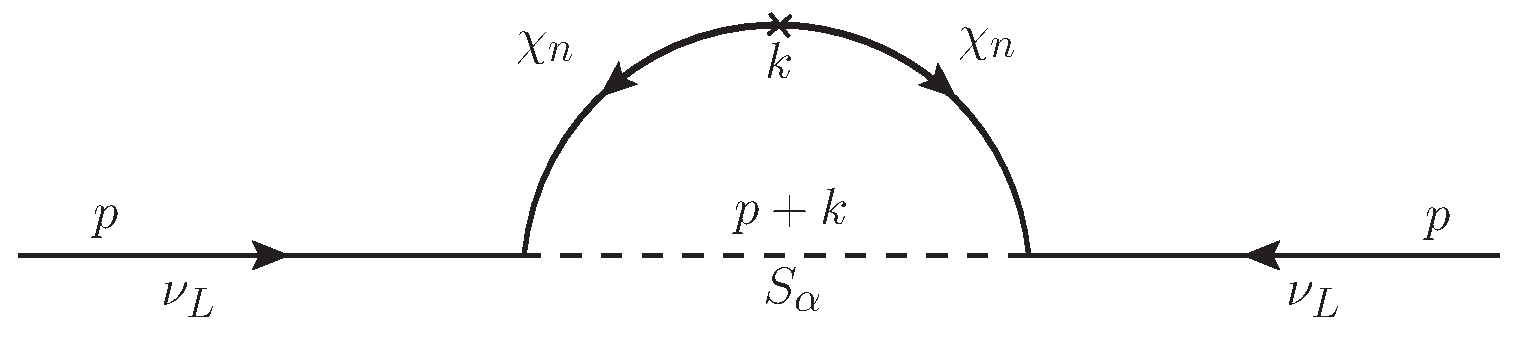
\includegraphics[scale=0.4]{neutrino_mass_diagram}
  \caption{Contributions to the neutrino mass matrix.}
  \label{fig:T13Aweylme}
\end{figure}
%
The neutrino mass matrix in this basis is given by
\begin{align*}
  M^{\nu}_{ij}=&i\sum_{\alpha}\int \frac{d^4k}{(2\pi)^4}\sum_{n=1}^3 \left( -i h_{i\alpha} N_{3n} \right) i S_F(k)\left( -i h_{j\alpha} N_{3n} \right)i\Delta_F(p+k)\nonumber\\
=&i\sum_{\alpha}\frac{h_{i\alpha}h_{j\alpha}}{16\pi^2}\sum_{n=1}^3 \left( N_{3n} \right)^2\int \frac{d^4k}{\pi^2}\frac{\cancel{k}+m_{\chi_n}}{\left(k^2-m_{\chi_n}^2  \right)\left[\left(p+k\right)^2-m_{S_\alpha}^2\right]}\,.
\end{align*}
In the limit of $p\to 0$, we have
\begin{align}
\label{eq:mnueig}
  M^{\nu}_{ij}=&i^2\sum_{\alpha}\frac{h_{i\alpha}h_{j\alpha}}{16\pi^2}\sum_{n=1}^3 \left( N_{3n} \right)^2m_{\chi_n}\; B_0 \left(0;m_{\chi_n}^2,m^2_{S_{\alpha}} \right)\,,
\end{align}
where $B_0$ is the Passarino Veltman functions given by~\cite{Passarino:1978jh}
%
\begin{align}
B_0 \left(0;m_{\chi_n}^2,m^2_{S_{\alpha}} \right)=&\int \frac{d^4k}{i\pi^2}\frac{1}{\left(k^2-m_{\chi_n}^2\right)\left(k^2-m_{S_\alpha}^2\right)}
=\frac{1}{m_{\chi_n}^2-m_{S_\alpha}^2}\left[ A_0\left(m_{\chi_n}^2\right)-A_0\left(m_{S_\alpha}^2\right)  \right] 
\end{align}
%
with
\begin{align}
A_0\left(m^2\right)=&\, m^2 \left[ \left( \frac{2}{\epsilon}-\ln\pi+\gamma_E \right)+1-\ln \left(\dfrac{m^2}{\mu^2} \right) \right] \,.
\end{align}

In order to compute this matrix, two things need to be used. 
First, the Eq.~\eqref{eq:mnueig}, where 
\begin{align}
\label{eq:mnueigdev}
\sum_{n=1}^3& \left( N_{3n} \right)^2m_{\chi_n}\; B_0 \left(0;m_{\chi_n}^2,m^2_{S_\alpha} \right)\nonumber\\
  &=\sum_{n=1}^3 \left( N_{3n} \right)^2m_{\chi_n}
   \left\{\frac{1}{m_{\chi_n}^2-m_{S_\alpha}^2}\left[m^2_{\chi_n} \left[ \Delta+1-\ln \left( m_{\chi_n}^2/\mu^2 \right) \right]   
-m_{S_\alpha}^2 \left[ \Delta+1-\ln \left( m_{S_\alpha}^2/\mu^2 \right) \right]\right] \right\}\nonumber\\
&=\sum_{n=1}^3 \left( N_{3n} \right)^2m_{\chi_n}
   \left\{(\Delta+1)+\frac{m_{S_\alpha}^2\ln \left( m_{S_\alpha}^2/\mu^2 \right)-m_{\chi_n}^2\ln \left( m_{\chi_n}^2/\mu^2 \right)}{m_{\chi_n}^2-m_{S_\alpha}^2} \right\}\nonumber\\
&=\sum_{n=1}^3 \left( N_{3n} \right)^2m_{\chi_n}
   \left\{\left[\Delta+1+\ln\left( \mu^2 \right) \right]+\frac{m_{S_\alpha}^2\ln \left( m_{S_\alpha}^2 \right)-m_{\chi_n}^2\ln \left( m_{\chi_n}^2 \right)}{m_{\chi_n}^2-m_{S_\alpha}^2} \right\}\,,
\end{align}
%
and second, the Eq.~\eqref{eq:chidiag}, where
%
\begin{align}
\label{eq:divcan}
\mathbf{N} \mathbf{M}^\chi_{\text{diag}}\mathbf{N}^{\operatorname{T}}=\mathbf{M}^\chi\Rightarrow \sum_mN_{lm}m_{\chi_m} N_{nm}=(M^\chi)_{ln}\,, \Rightarrow
  \sum_m N_{3m}^2m_{\chi_m}=(M^\chi)_{33}=0\,.
\end{align}
%
%The explicit expression for $\mathbf{M}^{\chi}$ was used for $l=n=3\,$~\eqref{eq:Mchi}.
 
Finally, using the Eq.~\eqref{eq:mnueigdev} and Eq.~\eqref{eq:divcan} the neutrino mass matrix takes the form
%
\begin{align}
\label{eq:neutrino-mass-matrix}
M^{\nu}_{ij}=&\sum_{\alpha}\frac{h_{i\alpha}h_{j\alpha}}{16\pi^2}\sum_{n=1}^3 \left( N_{3n} \right)^2m_{\chi_n}
\left[ \frac{m_{\chi_n}^2\ln \left( m_{\chi_n}^2 \right)-m_{S_\alpha}^2\ln \left( m_{S_\alpha}^2 \right)}{m_{\chi_n}^2-m_{S_\alpha}^2} \right]\,.
\end{align}






